\documentclass[a4paper,oneside,11pt]{book}
\usepackage{NWUStyle}
\usepackage{titlesec} % For redefining chapter title format
\usepackage{graphicx}
\usepackage{listings}
\graphicspath{ {./img/} }
% Redefine chapter and section spacing
\titlespacing{\chapter}{0pt}{-50pt}{5pt} % Adjust the spacing as needed
\titlespacing{\section}{0pt}{10pt}{5pt} % Adjust the spacing as needed
\setcounter{secnumdepth}{3}
\setcounter{tocdepth}{3}
\titleformat{\chapter}[display]
{\normalfont\huge\bfseries}{}{0pt}{\Huge}

\begin{document}
\Title{FITS Assignment}
\Initials{B.}
\FirstName{Bernard}
\Surname{Swanepoel}
\StudentNumber{39909476}
\Supervisor{Mr Henri van Rensburg}
\MakeTitle 
\pagenumbering{roman} 
\tableofcontents
\renewcommand{\thefigure}{\roman{figure}}
\pagenumbering{roman} 
\listoffigures
\cleardoublepage 
\pagenumbering{arabic} 

\chapter{Question 1}
\section{Introduction:}
In the realm of astronomical research and data management, the "Flexible Image Transport System (FITS)" stands as a cornerstone for storing and disseminating scientific data \citep{pence2010definition}. Developed in the late 1970s, FITS has evolved into a versatile and widely adopted standard for representing astronomical data and metadata \citep{pence2010definition}. Its flexibility and extensibility have made it indispensable for storing a diverse array of data types, ranging from images and spectra to tables and binary data \citep{pence2010definition}.

However, as the volume and complexity of astronomical data continue to expand exponentially, integrating FITS data into non-relational databases has emerged as a pressing challenge \citep{viswanatham2023big}. While relational databases have traditionally dominated data storage paradigms, the hierarchical and semi-structured nature of FITS data often aligns more closely with the principles of non-relational databases. Document stores, wide-column stores, and key-value stores offer promising alternatives for efficiently storing and querying FITS data, but navigating the intricacies of categorization and storage presents significant hurdles \citep{pattinson2022relational}.
\section{Problem statement:}
The integration of FITS data into non-relational databases poses significant challenges regarding categorization and storage methods. FITS data, characterized by its complexity and diverse structures, requires careful consideration of factors such as data volume, query complexity, and access patterns to ensure efficient storage and retrieval. Understanding these challenges and identifying optimal solutions is essential for facilitating seamless manipulation and analysis of FITS files within scientific research and data management environments, ultimately enhancing the usability and accessibility of astronomical data.
\section{Research question:}
How does the categorization of FITS data in the context of non-relational data types contribute to understanding potential storage methods in non-relational databases, and what factors influence the choice of these methods? Additionally, what features of the FITS data structure ensure data integrity, and how has the FITS file format evolved over time to meet the evolving needs of the scientific community, particularly in terms of data integrity and error prevention/correction?
\section{Aims:}
\begin{itemize}
    \item Understanding FITS Data Integration: The primary aim is to comprehend the integration of FITS  data into non-relational databases, exploring categorization, storage methods, and factors influencing these choices.
    \item Visualization and Explanation of FITS Structure: Another aim is to visualize and explain the complete structure of FITS components and extensions, focusing on accuracy and clarity to facilitate understanding.
    \item Evolution of FITS File Format: Understanding the historical evolution of the FITS file format to meet the evolving needs of the scientific community, highlighting key developments and their implications.
    \item Optimized Software Environment Design: Designing and illustrating a software environment optimized for the manipulation and analysis of FITS files using FITSIO, SAOImageDS9, and Miniforge3, with a focus on effectiveness and usability.
    \item Integration of Microservices: Exploring the use of microservices to improve the processing and analysis of FITS files, particularly integrating FITSIO, SAOImageDS9, and Miniforge3 into a microservices architecture for enhanced functionality.
    \item Designing a Microservice: Designing a microservice using the Flask web framework for Python and FITSIO to manipulate FITS files, including the development of a REST API for interaction, with a focus on modularity, security, and efficiency.
\end{itemize}
\section{Objectives:}
\begin{itemize}
    \item Investigate existing methods for integrating FITS data into non-relational databases.
    \item Analyze factors such as data volume, query complexity, and access patterns to determine optimal storage methods.
    \item Provide explainable content, such as diagrams and documentation, to clarify the purpose and organization of each component within a FITS file.
    \item Conduct a historical review of the development of the FITS file format, tracing key milestones and enhancements.
    \item Identify specific scientific needs and challenges that drove the evolution of FITS over time.
    \item Evaluate the impact of each major version or update of the FITS standard on data compatibility, accessibility, and usability.
    \item Define requirements for a software environment tailored to FITS file manipulation and analysis.
    \item Select and configure appropriate tools and libraries, such as FITSIO, SAOImageDS9, and Miniforge3, to meet the defined requirements.
    \item Investigate the principles and benefits of microservices architecture for FITS file processing and analysis.
    \item Identify specific functionalities of FITSIO, SAOImageDS9, and Miniforge3 that can be encapsulated as microservices.
    \item Develop integration strategies to orchestrate these microservices within a cohesive architecture, considering factors like scalability and fault tolerance.
    \item Define the scope and functionality of the microservice to be developed using Flask and FITSIO.
    \item Implement modular design patterns to facilitate future extension and maintenance of the microservice.
\end{itemize}
\section{How would you categorise FITS data in the context of non-relational data types? Discuss the potential ways FITS data could be stored in a non-relational database and the factors that might influence this choice.}
\subsection{Understanding of FITS data and non-relational data types.}
\subsubsection{FITS data type:}
The FITS data type was first introduced in the 1970s \citep{pence2010definition}. It outlined a universal method to encode both data definitions and the data itself in a manner independent of specific machine configurations, with magnetic tape serving as the standard transport medium \citep{grosbol1991fits}. With its introduction, the data type was widely accepted in different sectors of astrophysics \citep{pence2010definition}. 
Astrophysics often relies on this data format due to its compatibility with the archival systems used in most digital repositories of astronomical data \citep{pence2010definition}. Additionally, FITS stands out as one of the primary file formats utilized by analysis applications during runtime, and its relevance remains as an important part of data formats within the Virtual Observatory \citep{pence2010definition}.

Their are 5 types of FITS data type \citep{nass1999fits}:
\begin{itemize}
    \item "Unsigned 8-bit bytes" \citep{nass1999fits}.
    \item "16-bit Signed integers" \citep{nass1999fits}.
    \item "32-bit Signed integers" \citep{nass1999fits}.
    \item "32-bit Single or double precision floating point reals" \citep{nass1999fits}.
    \item "64-bit Single or double precision floating point reals" \citep{nass1999fits}.
\end{itemize}
In addition to this, FITS can store: "16 and 32-bit unsigned integers" \citep{nass1999fits}.
\subsubsection{Non-relational data type:}
Their are 5 types of non relational data types:
\begin{itemize}
    \item Document data stores:A document data store organizes a collection of named string fields and object data values within a structure known as a "document" \citep{pattinson2022relational}. These documents are commonly stored in formats such as XML, JSON, BSON, YAML, or plain text, offering adaptability in encoding methods \citep{pattinson2022relational}.
    \item Columnar (or column oriented) data stores: A columnar data store arranges data into columns, akin to the structure found in relational databases \citep{pattinson2022relational}. However, the primary advantage of a column-family database lies in its denormalized method of organizing sparse data, derived from its focus on storing data in a column-oriented fashion \citep{pattinson2022relational}.
    \item Key value stores: As the name suggests, a key-value store is essentially a repository of key-value pairs encapsulated within an object \citep{pattinson2022relational}.
    \item Document stores: Document stores present a higher level of complexity compared to key-value stores \citep{pattinson2022relational}. They do not presuppose a predefined document structure outlined by a schema \citep{pattinson2022relational}. Instead, document stores are engineered to accommodate documents in their natural form, enabling intricate querying processes \citep{pattinson2022relational}. MongoDB and CouchDB are examples of document stores \citep{pattinson2022relational}.
    \item Graph database: The most difficult among non-relational database types is the graph database \citep{pattinson2022relational}. It is specifically crafted to adeptly manage relationships between entities \citep{pattinson2022relational}. Graph databases are good in scenarios where data displays extensive interconnections, such as in purchasing and manufacturing systems or referencing catalogs \citep{pattinson2022relational}.
\end{itemize}
\pagestyle{plain}
\subsection{Appropriate categorisation of FITS data.}
FITS data can be classified into 3 different extensions \citep{pence2010definition}. These extensions are defined according to the FITS standard:
\begin{itemize}
    \item Image Extension: "A N-dimensional array of pixels, like in a primary array" \citep{pence2010definition}.
    \item ASCII Table Extension: "Rows and columns of data in ASCII character format" \citep{pence2010definition}.
    \item Binary Table Extension - "Rows and columns of data in binary representation" \citep{pence2010definition}.
\end{itemize}
\subsection{Discussion on potential storage methods in non-relational database for FITS data.}
\subsubsection{Document Store:}
\begin{itemize}
    \item Image Extension: FITS files containing image data could be stored as documents within a document store database. Each document would represent a FITS file, and the image data along with any associated metadata would be stored within the document.
    \item ASCII Table Extension: FITS files containing ASCII table data could be stored as documents within the document store database. Each document would represent a FITS file, and the ASCII table data along with any associated metadata would be stored within the document.
    \item Binary Table Extension: FITS files containing binary table data could  be stored as documents within the document store database, with each document representing a FITS file and the binary table data stored within.
\end{itemize}
\subsubsection{Wide-Column Store:}
\begin{itemize}
    \item Image Extension: FITS image data could be stored in a wide-column store database, with each row representing a FITS file and columns representing different attributes such as pixel values, metadata, etc.
    \item ASCII Table Extension: Similarly, FITS files containing ASCII table data could be stored in the wide-column store database, with each row representing a FITS file and columns representing the data and metadata.
    \item Binary Table Extension: FITS files with binary table data could also be stored in the wide-column store database, with each row representing a FITS file and columns containing the binary table data and associated metadata.
\end{itemize}
\subsubsection{Key-Value Store:}
\begin{itemize}
    \item Image Extension: In a key-value store, each FITS file could be stored as a key-value pair, where the key is the unique identifier for the file, and the value is the image data along with metadata.
    \item ASCII Table Extension: Similarly, FITS files containing ASCII table data could be stored as key-value pairs, with the key being the file identifier and the value being the ASCII table data and metadata.
    \item Binary Table Extension: FITS files with binary table data could also be stored as key-value pairs, with the key representing the file and the value containing the binary table data and associated metadata.
\end{itemize}
\subsection{Factors influencing the choice of storage method}
\begin{itemize}
    \item Data Structure and Schema: The structure of the data within the FITS files plays an important role. Document stores are good for storing complex, hierarchical data structures like FITS files, where each document can represent a complete FITS file with its associated metadata. Key-value stores are more appropriate for simpler data structures, where each file can be represented as a key-value pair.
    \item Query Requirements: Take into consideration the types of queries that will be performed on the data. Document stores give flexibility in querying nested structures, which can be a great attribute if you need to frequently query both the image data and metadata together \citep{greisen2002representations}. Key-value stores are efficient for simple retrieval by key but may not support complex querying as well as document stores. Wide-column stores offer the ability to query specific columns efficiently, which can be advantageous if your queries often involve a subset of attributes.
    \item Scalability: Document stores can scale horizontally by distributing documents across different nodes, which can handle large volumes of data and high read and write loads. Key-value stores  support horizontal scalability, making them suitable for large-scale applications. Wide-column stores offer scalability through distributed storage and are optimized for handling large amounts of data.
    \item Performance: Evaluate the performance characteristics of each storage method based on your specific use case. Document stores and wide-column stores are typically optimized for read-heavy workloads and can efficiently retrieve large volumes of data. Key-value stores excel in simple read and write operations, making them suitable for applications requiring high throughput.
\end{itemize}
\chapter{Question 2}
\section{Provide a visualisation and explain the complete structure of the FITS components and extensions.}
\subsection{Accurate visualisation of FITS components and extensions.}
\begin{figure}[h]
    \centering
    \makebox[\textwidth][c]{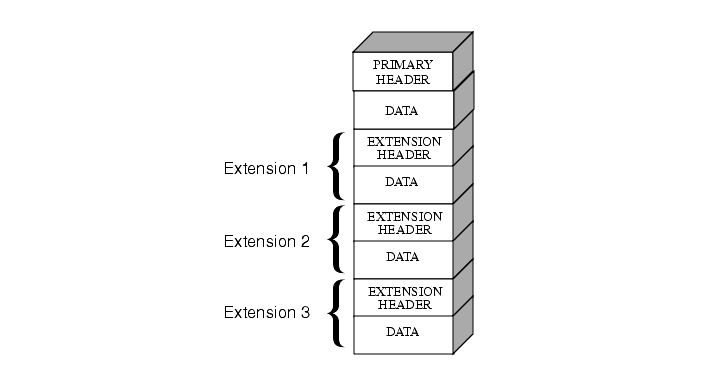
\includegraphics[width=1\textwidth, height=1\textheight, keepaspectratio]{format1.png}}
    \caption{Visualisation of FITS extensions and components \citep{fits_3}.}
\end{figure}
\begin{figure}[h]
    \centering
    \makebox[\textwidth][c]{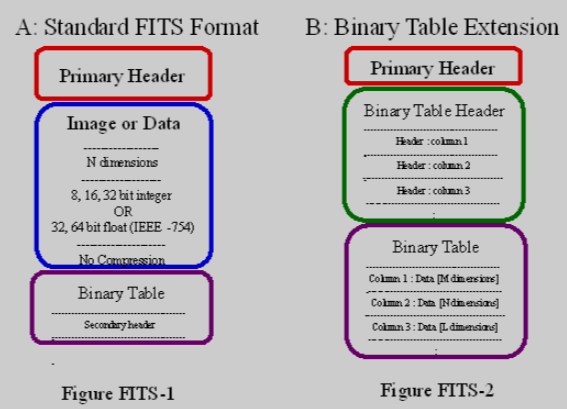
\includegraphics[width=0.7\textwidth, height=0.7\textheight, keepaspectratio]{format2.png}}
    \caption{Additional visualisation of FITS extensions and components \citep{fits_3}.}
\end{figure}
\subsection{Clear explanation of FITS components and extensions.}
\subsubsection{Components and extensions:}
\begin{itemize}
    \item Header and data units (HDUs): A FITS file consists out of the following: One or more header and data units, where the first HDU is called the primary array \citep{fits_3}. The primary array contains an N-dimensional array of pixels, such as a two-dimensional image, a one-dimensional spectrum, or a three-dimensional data cube \citep{fits_3}.
    \item Primary HDU: The primary HDU is empty or contains an array of pixels \citep{fits_3}. It is the starting point of a FITS file and sets the size and format of the following data unit \citep{fits_3}.
    \item Extensions: Additional HDUs can follow the primary array. Three types of extensions are included in the FITS standard \citep{nasa_fits_overview}:
    \begin{itemize}
        \item Image Extension: "An N-dimensional array of pixels, similar to the primary array" \citep{pence2010definition}.

        \item ASCII Table Extension: "Rows and columns of data in ASCII character format" \citep{pence2010definition}.
        
        \item Binary Table Extension: "Rows and columns of data in binary representation, with support for various numeric data types" \citep{pence2010definition}.
    \end{itemize}
    \item Header Records: Each HDU has a required keyword that specifies the size and format of the following data units \citep{fits_3}. Headers consist out of an eighty-character keyword record in a specific format \citep{fits_3}.
    \item Data Units: The data portion of an HDU, which follows the header \citep{fits_3}. It contains the actual data represented in the FITS file \citep{fits_3}.
    \item Reserved Keywords: Keywords in the header records that have predefined meanings are used to convey important metadata about the data stored in the FITS file \citep{fits_3}.
    \item User-Provided Keywords: Additional keywords that users can include in the header records to provide custom metadata about the data \citep{fits_3}.
    \item COMMENT and HISTORY Records: Optional records in the header that can be used to add comments or historical information about the data stored in the FITS file \citep{fits_3}.
\end{itemize}
\section{How does the FITS data structure you provided in question 2.1 ensure data integrity? What features does it have to prevent and correct errors?}
\subsection{Understanding of FITS structure.}
The FITS structure ensures data integrity through its well-defined components and extensions. By accurately visualizing FITS components and extensions, users can grasp the organization of data within a FITS file.

Figure i: Visualizes the primary components of FITS extensions and components \citep{fits_3}.

Figure ii: Provides additional visualization of FITS extensions and components \citep{fits_3}.

These figures aid in Understanding the hierarchical structure of FITS, including the primary HDU, extensions such as image, ASCII table, and binary table extensions, as well as header records, data units, reserved keywords, and user-provided keywords. Understanding these elements is crucial for effectively working with FITS files and ensuring data integrity.

\subsection{Explanation of how FITS ensures data integrity.}
\begin{itemize}
    \item Header Information: FITS files consist of Header and data units (HDUs). The header contains important metadata about the data, such as data types, dimensions, and calibration details \citep{fits_3}. This header information is stored in human-readable ASCII format, making it accessible \citep{fits_3}.
    \item Checksums: FITS files can include checksums to verify the integrity of the data \citep{seaman1995astronomical}. Checksums are calculated on what the file contains and can be used to detect any accidental or intentional modifications to the data.
    \item Backward Compatibility: FITS adheres to the principle of "once FITS, forever FITS" \citep{fits_3}. This means that backward compatibility is preserved even as new features are added \citep{fits_3}. This feature ensures that older FITS files remain readable and usable with newer software and systems \citep{fits_3}.
    \item Documentation: FITS is documented and maintained under the auspices of the International Astronomical Union (IAU) \citep{fits_3}. The format is well-defined and standardized, ensuring consistency and integration across different implementations and software libraries \citep{fits_3}.
    \item Community Practices: Astronomers and astrophysicists, who are the primary users of FITS, often follow community practices for documenting data quality and provenance \citep{fits_3}. This includes using keywords, comments, and history records within the FITS header to give additional context and information about the data \citep{fits_3}.
\end{itemize}
\subsection{Discussion on features preventing and correcting errors.}
\begin{itemize}
    \item Metadata and Self-Documentation: FITS provides a mechanic for metadata storage and self-documentation \citep{fits_3}. This allows users to include essential information about the data within the file itself \citep{fits_3}. This includes optional keyword/value records in headers, COMMENT and HISTORY records for additional documentation, and community practices \citep{fits_3}.
    \item Error logs: When errors occur during the reading, writing, or processing of FITS files, software libraries or applications provides detailed error messages or log entries \citep{fits_3}. This allows users to diagnose and troubleshoot issues more effectively, leading to prompt error correction and prevention of future occurrences \citep{fits_3}.
    \item Versioning and Updates: Although FITS follows a principle of "once FITS, forever FITS" to ensure backward compatibility, updates and revisions to the FITS standard can incorporate improvements, bug fixes, or clarifications to address known issues or errors \citep{fits_3}.
    \item Community Support and Best Practices: The FITS community provides support, resources, and best practices for users and developers working with FITS files \citep{fits_3}.
\end{itemize}
\section{Describe how the FITS file format evolved over time to meet the needs of the scientific community.}
\subsection{Understanding of FITS file format.}
FITS is a file format primarily designed for storing, transmitting, and manipulating scientific images and associated data, particularly in the field of astronomy \cite{fits_3}.
\subsubsection{File format summary:}
\begin{itemize}
    \item Type:	General data format \citep{fits}.
    \item Colors: Unlimited gray scale \citep{fits}.
    \item Compression: Uncompressed \citep{fits}.
    \item Multiple Images Per File: Yes \citep{fits}.
    \item Numerical Format: Two's complement/big-endian \citep{fits}.
    \item Originator: NOST \citep{fits}.
    \item Platform:	All \citep{fits}.
    \item Supporting Applications: FITSview, IMDISP, xv, pbmplus and SAOImage \citep{fits}.
\end{itemize}
\subsection{Detailed description of its evolution over time.}
The initial concept of FITS for astrophysics was proposed by two individuals: Greisen and Wells  in 1979 \citep{grosbol1991fits}. They suggested a method to encode both the data and data definitions in a universal manner, primarily using a "magnetic tape" as the main standard for transport mediums \citep{grosbol1991fits}. Recognizing the advantages of a standardized format for astronomical image transport, most large observatory' facilities adopted FITS as the primary structure for data exchange \citep{grosbol1991fits}.

In 1981, the FITS tape format, recommended by Wells and colleagues, was established as the standarlized style for image data interchange among observatories by "Commission 5" at the generalized assembly of the "International Astronomical Union (IAU)" in Patras \citep{grosbol1991fits}. During this assembly, the "first extension" of the FITS standard, known as the "random-groups" extension, was also recommended, allowing the transportation of numerous data matrices with non-uniform spacing \citep{grosbol1991fits}.

Subsequently, during discussions at the Patras gathering of "IAU Commission 5", the potential extension of FITS to encompass table and catalog data was explored \citep{grosbol1991fits}. This led to the formation of a "FITS Task Force" under the Working Group on "Astronomical Data" \citep{grosbol1991fits}. This task force was given the task to define and test a table extension to the FITS standard \citep{grosbol1991fits}. Their efforts combined into a proposed solution for "generalized extensions" to FITS, with a "special extension" adapted specifically for table and catalog data \citep{grosbol1991fits}.

Furthermore, guidelines were implemented to physically block logical FITS data entries into "2880-byte segments", aiming to enhance the efficiency of "high recording densities" and emerging data storage media such as "optical disks" and "helical scan cartridge tape devices" \citep{grosbol1991fits}. These FITS extensions were officially endorsed by the IAU General Assembly in "Baltimore" in 1988, which also mandated the establishment of a permanent "FITS Working Group" \citep{grosbol1991fits}.
\subsection{Discussion on how it meets the needs of the scientific community.}
\begin{itemize}
    \item Interoperability and Data Exchange: FITS emerged in response to the need for a standard format that could facilitate the exchange of astronomical data across different computing platforms.
    \item Long-Term Stability and Compatibility: FITS was designed with the principle of "once FITS, always FITS," emphasizing perpetual backward compatibility \citep{scroggins2020once}. 
    \item Community Governance: The governance structure surrounding FITS, led by international astronomical organizations such as the International Astronomy Union (IAU), provided a framework for collaborative decision-making and standardization \citep{scroggins2020once}.
    \item Flexibility and Adaptability: Despite its initial design decisions aimed at ensuring compatibility, FITS demonstrated a degree of flexibility by accommodating local modifications and workarounds \citep{greisen2002representations}. 
    \item Infrastructure for Circulation and Collaboration: FITS, along with associated communication channels like listservs and newsgroups, served as essential components of the astronomical infrastructure for data circulation and collaboration \citep{scroggins2020once}.
\end{itemize}
\chapter{Question 3}
\section{Design and illustrate a software environment and flow using FITSIO, SAOImageDS9, and Miniforge3 that optimizes the manipulation and analysis of FITS files.}
\subsection{Appropriate use of general systems' theory.}
\subsubsection{What is general theory.}
The creation of "general system theory (GST)" was attributed by Bertalanffy \citep{hofkirchner2011general}. GST is the investigation of general laws for comple arrangements (systems) \citep{sieniutycz2020systems}. 
\subsubsection{How will general theory be used in designing and illustrating.}
\begin{itemize}
    \item System thought process: GST encourages the view of the software environment as a complex system composed of interconnected components.
    \item System Topologies: GST provides principles for organizing system components into structured topologies.
    \item Conceptual Design: GST encourages developing high-level conceptual models that capture the essential features and behaviors of a system. 
    \item System Analysis and Optimization: GST provides methods for analyzing system behavior and optimizing its performance.
\end{itemize}
\subsection{Effective design and illustration of software environment.}
\subsubsection{Components:}
\begin{itemize}
    \item FITSIO:
    FITSIO is a library for reading and writing FITS files. It provides efficient and reliable functions for accessing FITS file data and metadata. FITSIO allows seamless integration of FITS file handling capabilities into software applications \citep{li2005introduction}.
    \item SAOImageDS9: SAOImageDS9 is a powerful and versatile astronomical imaging and data visualization tool \citep{SAOimageDSFeatures}. It supports the display and manipulation of FITS images, as well as various analysis tasks \citep{SAOimageDSFeatures}. SAOImageDS9 offers a user-friendly interface for exploring and interpreting FITS data \citep{SAOimageDSFeatures}.
    \item Miniforge3: Miniforge3 is a lightweight package manager for Python environments, based on conda. It provides a streamlined way to install and manage scientific computing packages, including those required for FITS file manipulation and analysis. Miniforge3 ensures compatibility and dependency management for Python-based tools and libraries.
\end{itemize}
\subsubsection{Design:}
\begin{itemize}
    \item Data collection: FITS files are collected from observatories, telescopes or other sources. FITSIO will be used to read and extract relevant data or metadata from the FITS files \citep{li2005introduction}.
    \item The preprocessing of data: Preprocessing could be followed to clean data. Example of this processing is bias subtraction. FITSIO facilitates Effective features  for preprocessing tasks \citep{li2005introduction}.
    \item Visualisation: Processed FITS images are visualized using SAOImageDS9. SAOImageDS9 provides interactive tools for exploring FITS images, adjusting display settings, and annotating features \citep{SAOimageDSFeatures}.
    \item Various analysis techniques spectroscopy and image processing are performed on the FITS data. Custom algorithms can be written to automate this process. Miniforge3 ensures that required Python packages, such as NumPy, SciPy, and Astropy, are installed and up to date.
    \item Result Interpretation: Analysis results are interpreted within the context of astronomy. SAOImageDS9 is used to overlay analysis results on FITS images for the purpose of visualization and comparison.
\end{itemize}
\newpage
\subsubsection{Illustrations:}
\begin{figure}[h]
    \centering
    \makebox[\textwidth][c]{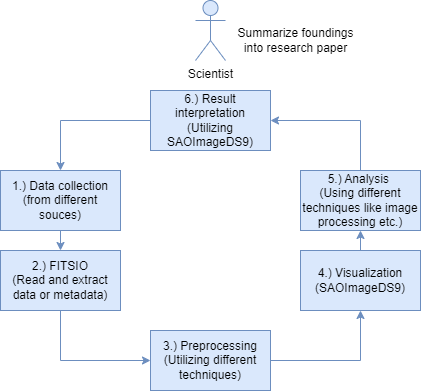
\includegraphics[width=1\textwidth, height=1\textheight, keepaspectratio]{FlowDiagram.png}}
    \caption{Visualisation of FITSIO, SAOImageDS9 and Miniforge3 working together.}
\end{figure}
\clearpage
\begin{figure}[h]
    \centering
    \makebox[\textwidth][c]{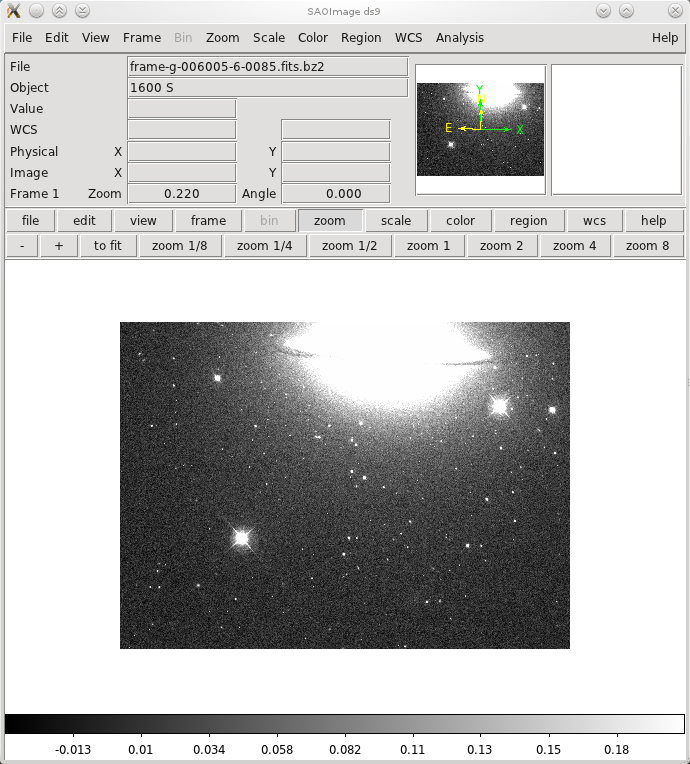
\includegraphics[width=1\textwidth, height=1\textheight, keepaspectratio]{ds91.png}}
    \caption{Visualisation of FITS Image in SAOImageDS9 \citep{sanders2011how}}
\end{figure}
\clearpage
\section{What considerations did you make when designing this environment?}
\subsection{Optimization of manipulation and analysis of FITS files.}
\begin{itemize}
    \item Efficient File Handling: FITSIO provides efficient functions for reading and writing FITS files, ensuring that data access and manipulation tasks are performed quickly and reliably.
    \item Streamlined Visualization: SAOImageDS9 offers a user-friendly interface for visualizing FITS images and conducting analysis tasks. Its interactive tools allow users to explore data effectively, enhancing the efficiency of analysis workflows.
    \item Custom Analysis Development: The Python ecosystem supported by Miniforge3 enables the development of custom analysis techniques tailored to specific scientific objectives. Researchers can leverage Python's extensive scientific computing libraries to implement sophisticated analysis algorithms efficiently.
    \item Visualization and Interpretation: SAOImageDS9's visualization tools enhance the interpretation of analysis results by providing interactive features for annotating features, overlaying analysis results on images, and comparing different datasets. 
    \item Integration of Preprocessing Steps: FITSIO facilitates the integration of preprocessing steps into the analysis workflow.
\end{itemize}
\subsection{Considerations made when designing the environment.}
\begin{itemize}
    \item Usability: The software environment was designed to be user-friendly, allowing astronomers to easily navigate and interact with FITS files.
    \item Integration: The environment integrates multiple tools and libraries, such as FITSIO, SAOImageDS9, and Miniforge3, to provide a comprehensive solution for FITS file manipulation and analysis.
    \item The environment offers a wide range of functionality, including data collection, preprocessing, visualization, analysis, and result interpretation. 
    \item Performance: Considerations were made to optimize the performance of the software environment, ensuring fast and efficient processing of FITS files. 
    \item Flexibility: The environment was designed to be flexible and adaptable to different use cases and research needs. 
    \item Documentation: Comprehensive documentation and support resources were provided to assist users in effectively utilizing the software environment.
\end{itemize}
\chapter{Question 4}
\section{How can microservices be used to improve the processing and analysis of FITS files using FITSIO, SAOImageDS9 and Miniforge3?}
\subsection{Understanding of microservices.}

A microservices represent both a structural and procedural methodology in software development \citep{microservices}. In this paradigm, applications are constructed from numerous autonomous services, each fulfilling specific functions and communicating via clearly defined APIs \citep{microservices}. Each service operates within its own codebase, manageable by a compact development team \citep{ozkaya2021microservices}. One of the key advantages of microservices is that they are independently deployable \citep{ozkaya2021microservices}. Teams can update individual services without the need to rebuild and redeploy the entire application \citep{ozkaya2021microservices}. Furthermore, each service is responsible for managing its own data or external state \citep{ozkaya2021microservices}. This stands in contrast to traditional architectures where a centralized data layer handles data persistence \citep{ozkaya2021microservices}.
\noindent
\subsection{Discussion on how microservices improve processing and analysis of FITS files.}
\begin{itemize}
    \item Scalability: Microservices architecture allows for scaling different components independently based on demand \citep{ferreira2023microservices}. For FITS file processing (which are large files), this means you can scale up services responsible for intensive tasks like data extraction or image analysis without affecting other parts of the system \citep{ferreira2023microservices}.
    \item Modularity and Flexibility: Each microservice can focus on a specific aspect of FITS file processing.
    \item Parallel Processing: Microservices can be designed to handle multiple FITS files concurrently, enabling parallel processing of large datasets \citep{stefanova2024spring}.
    \item Resource Optimization: Microservices can be deployed on containerized platforms like Docker or Kubernetes, allowing efficient utilization of computing resources \citep{h2023containerized}. 
    \item Service Orchestration: Microservices architecture facilitates complex workflows and pipelines for FITS file processing through service orchestration tools like Apache Airflow or Kubernetes-based workflows \citep{dey2023apache}.
    \item Fault Isolation and Resilience: Microservices keep problems contained. So, if something goes wrong with one microservice, it doesn't crash the whole system.
    \item Integration with External Systems: Microservices can easily integrate with external cloud services. This allows data exchange and operation between FITS file processing applications and other systems.
    \item Real-time Data Processing: Real-time Data Processing for time-sensitive applications.
\end{itemize}
\subsection{Use of FITSIO, SAOImageDS9, and Miniforge3 in the context of microservices and why it is better to integrate microservices.}
\begin{itemize}
    \item Modularization: Break down the processing and analysis tasks into smaller, independent modules or microservices. Integrating FITSIO, SAOImageDS9, and Miniforge3 within a microservices architecture promotes modularity and maintainability of the system. Each microservice focuses on a specific aspect of FITS file processing and analysis. 
    \item Scalability: Microservices architecture allows for horizontal scalability, meaning you can scale individual components independently based on the workload. FITSIO, SAOImageDS9, and Miniforge3 can each be encapsulated within separate microservices, allowing for fine-grained scalability.
    \item Integration with FITSIO: Develop microservices that interact with FITSIO. These microservices can handle tasks such as parsing FITS headers, extracting data arrays, or writing new FITS files.
    \item Integration with SAOImageDS9: Create microservices that integrate with SAOImageDS9. These microservices can generate image data from FITS files, apply image processing filters, and communicate with SAOImageDS9 for real-time visualization and analysis.
    \item Integration with Miniforge3: Utilize Miniforge3, a distribution of the conda package manager optimized for scientific computing, to manage dependencies and environments for the microservices. Each microservice can specify its own set of dependencies, which facilitates reuse and consistency across different environments.
    \item Asynchronous Processing: Microservices interacting with FITSIO, SAOImageDS9, and Miniforge3 can benefit from asynchronous processing for computationally intensive tasks, such as image processing or data analysis For example, a microservice responsible for image manipulation using SAOImageDS9 can asynchronously handle multiple image processing requests concurrently without blocking the execution flow. 
    \item API Gateway: An API gateway can be implemented to provide a unified interface for accessing microservices that interact with FITSIO, SAOImageDS9, and Miniforge3. The API gateway handles authentication, load balancing, and routing of requests to the appropriate microservices based on their capabilities and availability.
\end{itemize}
\section{Design a microservice using the Flask web framework for Python and FITSIO to manipulate FITS files. Your design should include a REST API for interacting with the microservice. Provide screenshots and/or code snippets demonstrating your working microservice where possible.}
\subsection{Effective design of a microservice.}
\subsubsection{Overall Architecture:}
\begin{itemize}
    \item The microservice will be implemented using the Flask web framework for Python.
    \item FITSIO, a library for reading and writing FITS files, will be integrated into the microservice for FITS file manipulation.
\end{itemize}
\subsubsection{REST API Design:}
\begin{itemize}
    \item The microservice will expose a RESTful API to interact with FITS files.
    \item API endpoints will be designed to perform operations such as opening, writing, reading, appending, renaming, and deleting FITS files.
    \item Each endpoint will handle specific functionalities related to FITS file manipulation.
\end{itemize}
\subsubsection{Endpoints:}
\begin{itemize}
    \item \texttt{/fits/open}: Endpoint to open a FITS file and return its header information.
    \item \texttt{/fits/write}: Endpoint to write a FITS file with provided data.
    \item \texttt{/fits/append}: Endpoint to append data to an existing FITS file.
    \item \texttt{/fits/read}: Endpoint to read the contents of a FITS file and return it.
    \item \texttt{/fits/rename/<new\_filename>}: Endpoint to rename the existing FITS file on the server.
    \item \texttt{/fits/delete}: Endpoint to delete the existing FITS file from the server.
\end{itemize}
\subsubsection{Error Handling:}
\begin{itemize}
    \item Robust error handling will be implemented to handle various scenarios, such as invalid requests or file operations.
    \item Error responses will include appropriate HTTP status codes and error messages for easy troubleshooting.
\end{itemize}
\subsubsection{Additional features:}
\begin{itemize}
    \item CORS (Cross-Origin Resource Sharing) support will be enabled to allow cross-origin requests.
    \item Configuration for the upload folder will be provided, specifying the directory where FITS files will be stored.
\end{itemize}
\subsubsection{Design illustration:}
\begin{figure}[h]
    \centering
    \makebox[\textwidth][c]{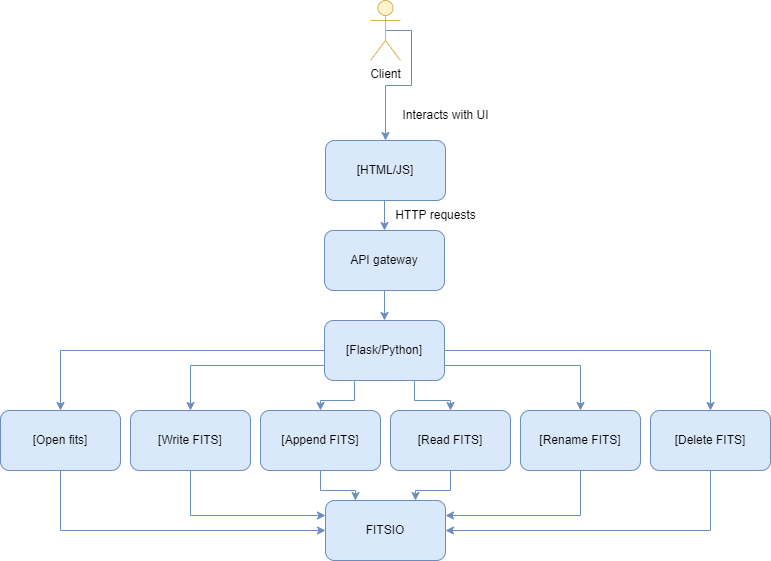
\includegraphics[width=1.2\textwidth, height=1.2\textheight, keepaspectratio]{FlaskAPIHTMLDesign.png}}
    \caption{Design illustration (the API gateway is the REST API) \citep{fits_3}.}
\end{figure}
\subsection{Inclusion of a REST API for interaction.}
\subsubsection{Endpoints and code:}
\begin{itemize}
    \item \texttt{/fits/open:}
    \begin{lstlisting}[language=Python, caption={Endpoint to open a FITS file}]
"@app.route('/fits/open', methods=['POST'])
def open_fits_file():
file = request.files.get('file')
if file and file.filename.endswith('.fits'):
try:
file.save(os.path.join(app.config['UPLOAD_FOLDER'], UPLOAD_FILENAME))
header_info = {}
with fitsio.FITS(os.path.join(app.config['UPLOAD_FOLDER']
, UPLOAD_FILENAME)) as fits:
header = fits[0].read_header()
header_info = {
'SIMPLE': header.get('SIMPLE', ''),
'NAXIS': header.get('NAXIS', ''),
'OBJECT': header.get('OBJECT', ''),
}
except Exception as e:
return jsonify({'error': str(e)}), 500
return jsonify({'header': header_info}), 200
else:
return jsonify({'error': 'No FITS file uploaded or file upload failed'}
), 400"
    \end{lstlisting}
    \item \texttt{/fits/write:}
    \begin{lstlisting}[language=Python, caption={Endpoint to rewrite a FITS file}]
"@app.route('/fits/write', methods=['POST'])
def write_fits_file():
data = request.json.get('data')
if data:
try:
fits_data = parse_input_data(data)
fitsio.write(os.path.join(app.config['UPLOAD_FOLDER']
, UPLOAD_FILENAME), fits_data, clobber=True)
except Exception as e:
return jsonify({'error': str(e)}), 500
return jsonify({'message': 'FITS file successfully written'}), 200
else:
return jsonify({'error': 'No data provided to write FITS file'}), 400"
    \end{lstlisting}
    \item \texttt{/fits/append:}
    \begin{lstlisting}[language=Python, caption={Endpoint to append to a FITS file}]
"@app.route('/fits/append', methods=['POST'])
def append_fits_file():
data = request.json.get('data')
if data:
try:
existing_fits_data = []
if os.path.exists(os.path.join(app.config['UPLOAD_FOLDER'],
UPLOAD_FILENAME)):
existing_fits_data = fitsio.read(os.path.join(
app.config['UPLOAD_FOLDER'], UPLOAD_FILENAME)).tolist()
combined_data = append_to_fits_file
(existing_fits_data, data)
fitsio.write(os.path.join(app.config['UPLOAD_FOLDER']
, UPLOAD_FILENAME), combined_data, clobber=True)
except Exception as e:
return jsonify({'error': str(e)}), 500
return jsonify({'message': 'Data successfully appended to FITS file'
}), 200
else:
return jsonify({'error': 'No data provided to append to FITS file'
}), 400"
    \end{lstlisting}
    \item \texttt{/fits/read:}
    \begin{lstlisting}[language=Python, caption={Endpoint to read a FITS file}]
"@app.route('/fits/read', methods=['GET'])
def read_fits_file():
try:
data = fitsio.read(os.path.join(app.config['UPLOAD_FOLDER']
, UPLOAD_FILENAME)).tolist()
except Exception as e:
return jsonify({'error': str(e)}), 500
return jsonify({'data': data}), 200"
    \end{lstlisting}
    \item \texttt{/fits/rename/<new\_filename>:}
    \begin{lstlisting}[language=Python, caption={Endpoint to rename a FITS file}]
"@app.route('/fits/rename/<string:new_filename>', methods=['PUT'])
def rename_fits_file(new_filename):
global UPLOAD_FILENAME
try:
if not new_filename.endswith('.fits'):
new_filename += '.fits'
old_file_path = os.path.join(app.config['UPLOAD_FOLDER']
, UPLOAD_FILENAME)
new_file_path = os.path.join(app.config['UPLOAD_FOLDER']
, new_filename)
if os.path.exists(old_file_path):
os.rename(old_file_path, new_file_path)
UPLOAD_FILENAME = new_filename
return jsonify({'message': 'FITS file successfully renamed'}), 200
else:
return jsonify({'error': 'FITS file not found'}), 404
except Exception as e:
return jsonify({'error': str(e)}), 500"
    \end{lstlisting}
    \item \texttt{/fits/delete:}
    \begin{lstlisting}[language=Python, caption={Endpoint to delete FITS file}]
"@app.route('/fits/delete', methods=['DELETE'])
def delete_fits_file():
try:
file_path = os.path.join(app.config['UPLOAD_FOLDER'], UPLOAD_FILENAME)
if os.path.exists(file_path):
os.remove(file_path)
return jsonify({'message': 'FITS file successfully deleted'}), 200
else:
return jsonify({'error': 'FITS file not found'}), 404
except Exception as e:
return jsonify({'error': str(e)}), 500"
    \end{lstlisting}
    \end{itemize}
\subsection{Screenshots demonstrating the working microservice.}
\begin{itemize}
    \newpage
    \item UI:
    \begin{figure}[h]
        \centering
        \makebox[\textwidth][c]{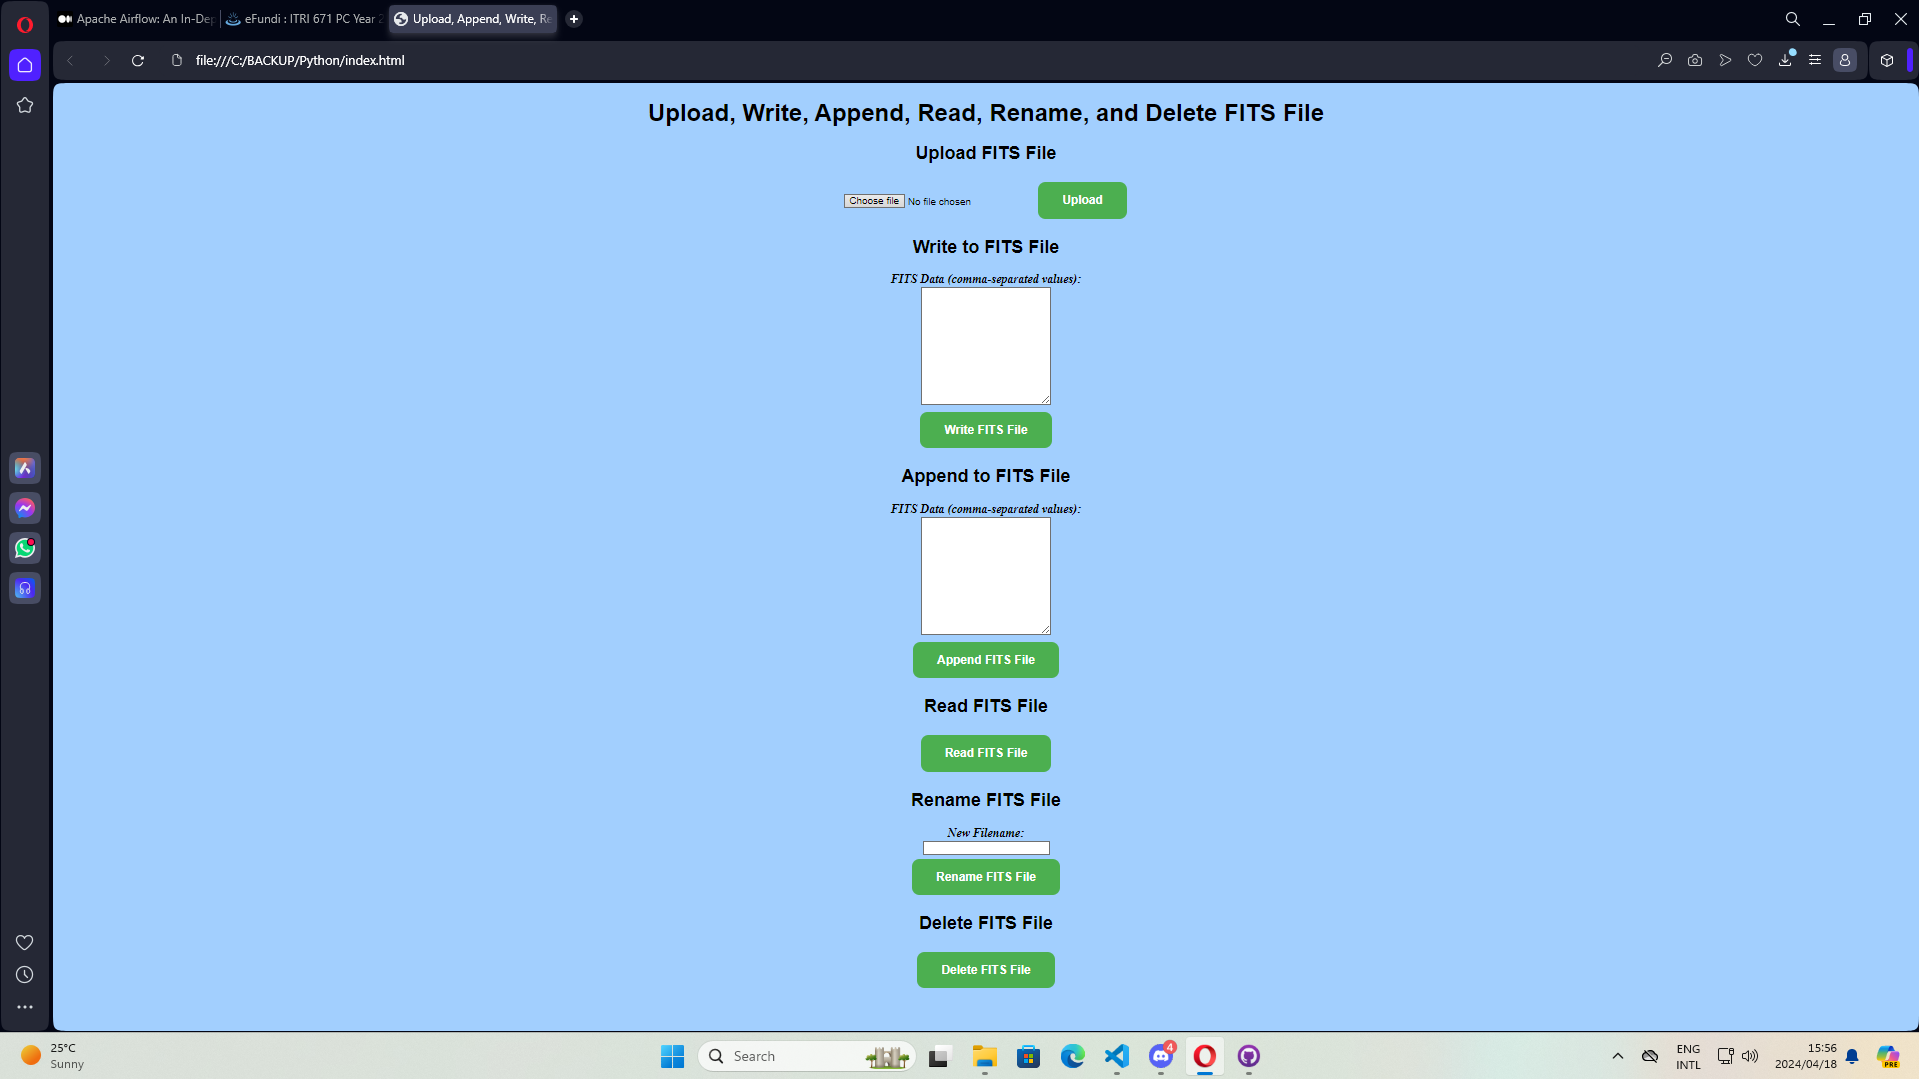
\includegraphics[width=1\textwidth, height=1\textheight, keepaspectratio]{showingUI.png}}
        \caption{User interface}
    \end{figure}
    \clearpage
    \item \texttt{/fits/open}:
    \begin{figure}[h]
        \centering
        \makebox[\textwidth][c]{
\includegraphics[width=1.3\textwidth, height=1.3\textheight, keepaspectratio]{ShowingSelectionOfFiles.png}}
        \caption{Selection of files}
    \end{figure}
    \begin{figure}[h]
        \centering
        \makebox[\textwidth][c]{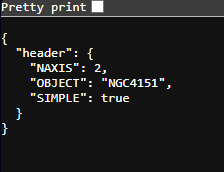
\includegraphics[width=1\textwidth, height=1\textheight, keepaspectratio]{ShowingHeaderInformationWhenUploaded.png}}
        \caption{Information of file is shown when uploaded}
    \end{figure} 
    \clearpage
    \item \texttt{/fits/write}:
    \begin{figure}[h]
        \centering
        \makebox[\textwidth][c]{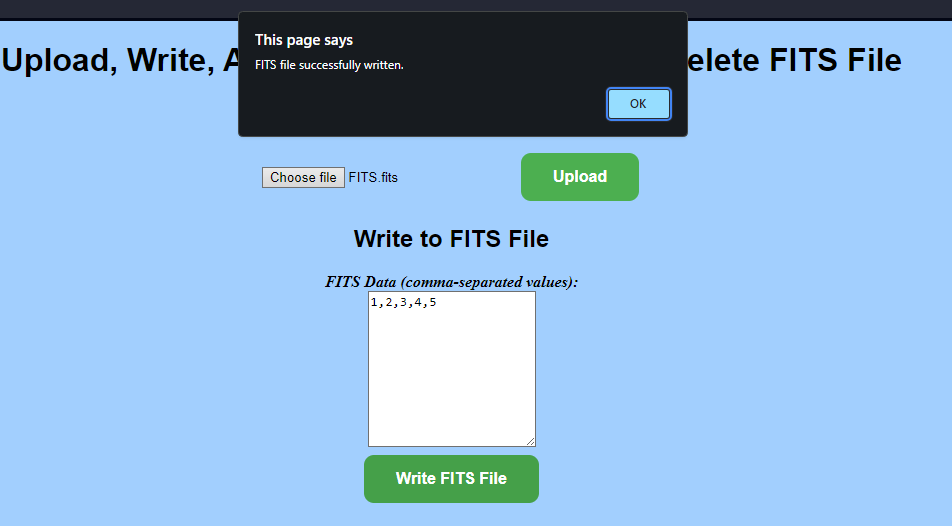
\includegraphics[width=1.3\textwidth, height=1.3\textheight, keepaspectratio]{ShowingWriteFileSucessful.png}}
        \caption{Write to file sucessful}
    \end{figure}
    \begin{figure}[h]
        \centering
        \makebox[\textwidth][c]{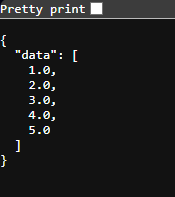
\includegraphics[width=0.5\textwidth, height=0.5\textheight, keepaspectratio]{ShowingWriteFileOutput.png}}
        \caption{Write to file output}
    \end{figure}
    \clearpage
    \item \texttt{/fits/append}: 
    \begin{figure}[h]
        \centering
        \makebox[\textwidth][c]{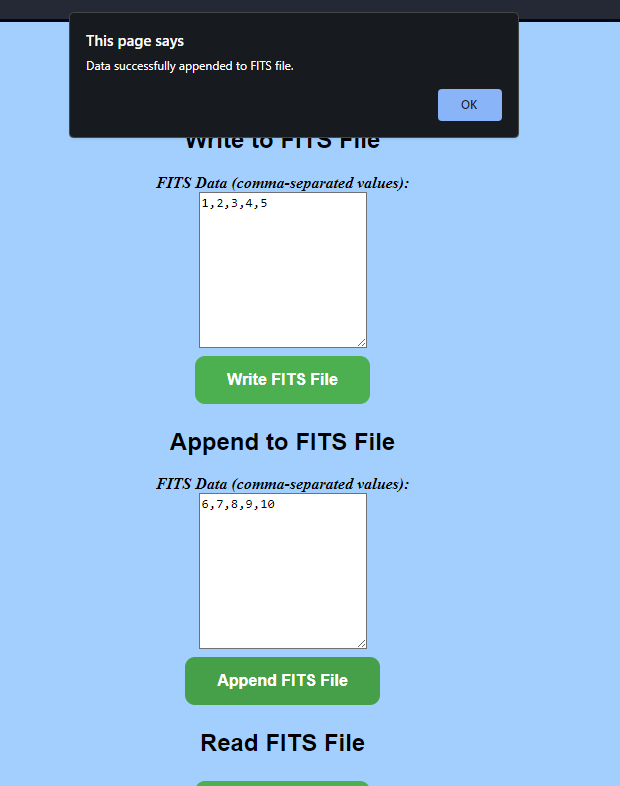
\includegraphics[width=0.7\textwidth, height=0.7\textheight, keepaspectratio]{ShowingAppendFileSucessful.png}}
        \caption{Append to file sucessful}
    \end{figure}
    \begin{figure}[h]
        \centering
        \makebox[\textwidth][c]{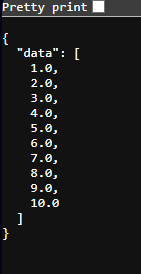
\includegraphics[width=0.5\textwidth, height=0.5\textheight, keepaspectratio]{ShowingAppendFileSucessfulOutput.png}}
        \caption{Output of append to file}
    \end{figure}
    \clearpage
    \item \texttt{/fits/rename/<new\_filename>}: 
    \begin{figure}[h]
        \centering
        \makebox[\textwidth][c]{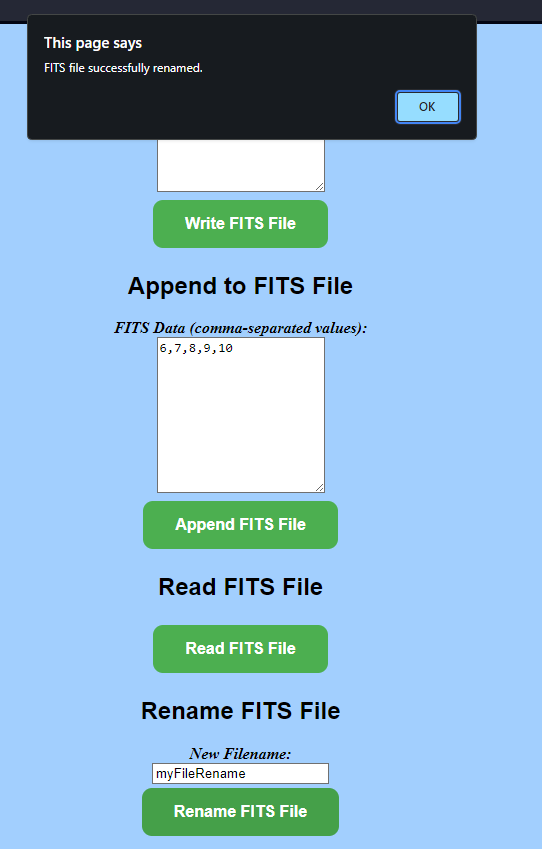
\includegraphics[width=0.7\textwidth, height=0.7\textheight, keepaspectratio]{ShowingRenameFileSucessful.png}}
        \caption{Rename file sucessful}
    \end{figure}
    \begin{figure}[h]
        \centering
        \makebox[\textwidth][c]{
\includegraphics[width=1.3\textwidth, height=1.3\textheight, keepaspectratio]{ShowingRenameFileSucessfulOutput.png}}
        \caption{Rename file output}
    \end{figure}
    \clearpage
    \item \texttt{/fits/delete}: 
    \begin{figure}[h]
        \centering
        \makebox[\textwidth][c]{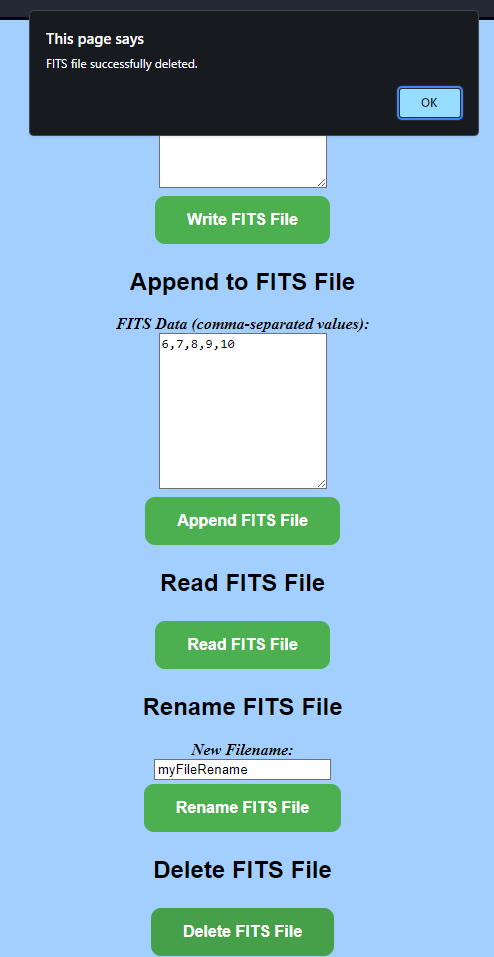
\includegraphics[width=0.7\textwidth, height=0.7\textheight, keepaspectratio]{ShowingDeleteFileSucessful.png}}
        \caption{File delete sucessful}
    \end{figure}
    \begin{figure}[h]
        \centering
        \makebox[\textwidth][c]{
\includegraphics[width=1.3\textwidth, height=1.3\textheight, keepaspectratio]{ShowingDeleteFileSucessfulOutput.png}}
        \caption{File delete output}
    \end{figure}
    \clearpage
    \item \texttt{Extra information:}
    \begin{figure}[h]
        \centering
        \makebox[\textwidth][c]{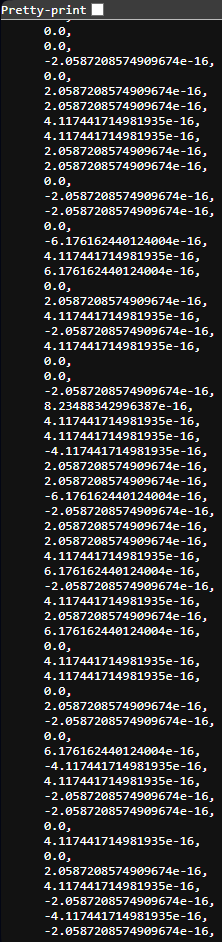
\includegraphics[width=0.7\textwidth, height=0.7\textheight, keepaspectratio]{output of read of full document.png}}
        \caption{Read of a NASA file as example}
    \end{figure}
    \begin{figure}[h]
        \centering
        \makebox[\textwidth][c]{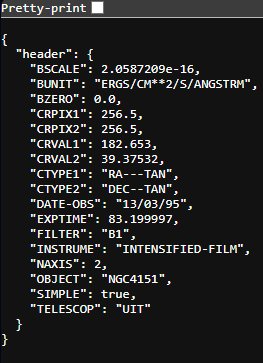
\includegraphics[width=0.7\textwidth, height=0.7\textheight, keepaspectratio]{extraheaders.png}}
        \caption{Additional header information}
    \end{figure}
    \clearpage
\end{itemize}
\section{In addition to designing a microservice using the Flask web framework for Python and
FITSIO to manipulate FITS files, describe the specific functionalities this microservice
will have. How will it interact with other microservices in your system? Provide
examples and explanations to support your design decisions.}
\subsection{Description of specific functionalities of the microservice.}
\subsubsection{\texttt{/fits/open}}
\begin{itemize}
    \item This endpoint accepts a POST request with a FITS file as input.
    \item It saves the uploaded FITS file to the specified upload folder.
    \item Then, it reads the header information of the FITS file and returns some common header keywords as JSON.
\end{itemize}
\subsubsection{\texttt{/fits/write}:}
\begin{itemize}
    \item This endpoint accepts a POST request with JSON data containing numerical values.
    \item It parses the input data and writes it to a new FITS file in the upload folder.
\end{itemize}
\subsubsection{\texttt{/fits/open}:}
\begin{itemize}
    \item This endpoint accepts a POST request with JSON data containing numerical values.
    \item It reads the existing FITS file (if any), parses the input data, and appends it to the existing FITS data.
    \item The combined data is then written back to the FITS file in the upload folder.
\end{itemize}
\subsubsection{\texttt{/fits/append}:}
\begin{itemize}
    \item This endpoint accepts a GET request.
    \item It reads the contents of the existing FITS file and returns the data as a list in JSON format.
\end{itemize}
\subsubsection{\texttt{/fits/rename}:}
\begin{itemize}
    \item This endpoint accepts a PUT request with a new filename as part of the URL path.
    \item It renames the existing FITS file to the provided filename.
\end{itemize}
\subsubsection{\texttt{/fits/delete}:}
\begin{itemize}
    \item This endpoint accepts a DELETE request.
    \item It deletes the existing FITS file from the server.
\end{itemize}
\subsubsection{Cross-Origin Resource Sharing (CORS) Support:}
\begin{itemize}
    \item The microservice utilizes the flask cors extension to enable Cross-Origin Resource Sharing. This allows clients from different origins to make requests to the microservice, which can be useful when developing web applications with client-side JavaScript.
\end{itemize}
\subsubsection{Debug Mode}
\begin{itemize}
    \item The microservice is configured to run in debug mode (debug=True) when executed directly. Debug mode provides additional information and error messages in the Flask application console, which can aid in development and debugging processes.
\end{itemize}
\subsection{Explanation of how it interacts with other microservices.}
\subsubsection{File Upload and create ({/fits/open} and {fits/write})}
\begin{itemize}
    \item Other microservices can send a FITS file to this service using a POST request to {/fits/open}. The service saves the file locally and extracts header information, which can be useful metadata about the FITS file.
    \item If other microservices want to create a new FITS file, they can send data in a JSON format to {/fits/write}. The service converts this data into FITS format and saves it as a new FITS file.
\end{itemize}
\subsubsection{File read {fits/read}}
\begin{itemize}
    \item Other microservices can retrieve the data stored in a FITS file by sending a GET request to {/fits/read}. The service reads the FITS file and returns the data in JSON format.
\end{itemize}
\subsubsection{File Management ({/fits/rename/} and {/fits/delete})}
\begin{itemize}
    \item Other microservices can rename a FITS file by sending a PUT request to {/fits/rename}. They provide the new filename in the URL, and the service renames the FITS file accordingly.
    \item If other microservices need to delete a FITS file, they can send a DELETE request to {/fits/delete}. The service removes the specified FITS file from the local storage.
\end{itemize}
\subsection{Examples and explanations supporting design decisions.}
\subsubsection{Security consideration:}
The application uses the os.path.join() function to construct file paths, which helps prevent path traversal attacks by securely joining directory paths.
\subsubsection{Flexibility and Configurability}
The code defines configurable parameters such as the upload folder and filename, allowing users to customize these settings based on their requirements.
\subsubsection{Use of try catch blocks:}
The code uses try-except blocks to catch and handle exceptions gracefully. For instance, when reading or writing FITS files, exceptions such as IOError or ValueError may occur. Catching these exceptions allows the application to return informative error messages to clients instead of crashing or leaking sensitive information.
\subsubsection{Input Data Validation:}
The code validates input data to ensure it meets the expected format. For example, the parseinputdata() function checks that input data for writing or appending FITS files consists of comma-separated numeric values. 
\section{Concluscion:}
In conclusion, the exploration of FITS data and its integration into non-relational databases reveals a important understanding of scientific data management. This report covered categorization within non-relational data types, potential storage methods, visualization of FITS components, data integrity assurance, FITS file format evolution, and optimized software environments for FITS manipulation.

FITS data's adaptability across various storage methods shows its versatility, while the structured nature of FITS files ensures data integrity and facilitates error prevention. The iterative development of the FITS formats reflects a commitment to meeting scientific community needs.

Optimized software environments, leveraging microservices and RESTful APIs, offer scalability and modularity, enhancing FITS-related workflows. The development of microservices using Flask and FITSIO demonstrates practical FITS manipulation functionalities with a focus on modularity and security.

In summary, the analysis emphasizes the importance of thoughtful design and alignment with scientific needs in FITS data management. By utilizing modern technologies, researchers can efficiently leverage FITS data for scientific discovery and advancement.
\bibliography{MyBib}
\end{document}
